\chapter{نظرة أولى إلى الخلايا}\label{ch:g5:first-look-at-cells}

انظر إلى ظاهر يدك: \omterm{def:g1:the-five-senses:sense}{جلد} أملس، وسطح واحد بلا فواصل. والآن تخيّل
عدسة مكبّرة قوية بما يكفي لتقريب ألف مرة. عندئذ ينحلّ السطح الأملس
إلى رصيف من حجيرات صغيرة، مركّبة بعضها إلى بعض كبلاط الأرض ---
وكل \omterm{def:g1:living-or-not:living}{كائن حي} لقيته في هذا الكتاب، من الطحلب إلى الحوت، مرصوف
الرصف نفسه. فأكبر أسرار \omterm{def:g1:living-or-not:living}{علم الأحياء} صغير.

\section{الكائنات الحية مصنوعة من خلايا}

\begin{definition}[الخلية]\label{def:g5:first-look-at-cells:cell}
\emph{الخلية}\index{خلية} أصغر لَبِنة حية في \omterm{def:g1:living-or-not:living}{الكائن الحي}. وأكثر
الخلايا أصغر بكثير من أن تُرى \omterm{def:g1:the-five-senses:sense}{بالعين} المجردة؛ والجسم مبني منها كما
يُبنى الجدار من الطوب. وجسمك أنت مصنوع من عشرات آلاف المليارات من
الخلايا.
\end{definition}

\begin{proposition}[مبدأ الخلية]\label{prop:g5:first-look-at-cells:principle}
كل \omterm{def:g1:living-or-not:living}{كائن حي} مصنوع من \omterm{def:g5:first-look-at-cells:cell}{خلايا} --- كل \omterm{def:g1:animals-around-us:animal}{حيوان}، وكل \omterm{def:g1:plants-around-us:plant}{نبات}، وكل فطر، حتى
الكائنات الحية التي ليست إلا \omterm{def:g5:first-look-at-cells:cell}{خلية} \emph{واحدة}. وهذا البناء
المشترك من أكبر علامات \emph{وحدة الحياة}\index{وحدة الحياة}:
فمهما تختلف الأقحوانة والحوت، فهما عن قرب مبنيان من الصنف نفسه من
الوحدات الحية الصغيرة.
\end{proposition}
\admitted

\begin{example}[ما مقدار هذا الصغر؟]\label{ex:g5:first-look-at-cells:small}
\omterm{def:g5:first-look-at-cells:cell}{خلية} معتادة من \omterm{def:g5:first-look-at-cells:cell}{خلايا} جسمك تبلغ نحو جزء من خمسين من المليمتر. فصفّ
$50$ منها فتمتد مليمترًا واحدًا --- ونقطة قلم رصاص تستطيع أن تغطي
الاستعراض كله. ولهذا لم يشك أحد في وجود \omterm{def:g5:first-look-at-cells:cell}{الخلايا} في معظم تاريخ
البشر: فلبنات الحياة أصغر من أصغر ذرّة تراها \omterm{def:g1:the-five-senses:sense}{العين}.
\end{example}

\section{الآلة التي كشفتها}

\begin{definition}[المجهر]\label{def:g5:first-look-at-cells:microscope}
\emph{المجهر}\index{مجهر} آلة تكبّر عدساتها الأشياء الشديدة الصغر
مئات المرات. وقد كشف، إذ وُجّه إلى شرائح رقيقة من مادة حية، ما لم
تره \omterm{def:g1:the-five-senses:sense}{عين} قط: \omterm{def:g5:first-look-at-cells:cell}{الخلايا}. والاسم نفسه صاغه راصد قديم رأى أن الحجيرات
الصغيرة في شريحة من الفلّين تشبه غرف الرهبان الصغيرة ---
\emph{\omterm{def:g5:first-look-at-cells:cell}{الخلايا}}.
\end{definition}

\begin{omfigure}
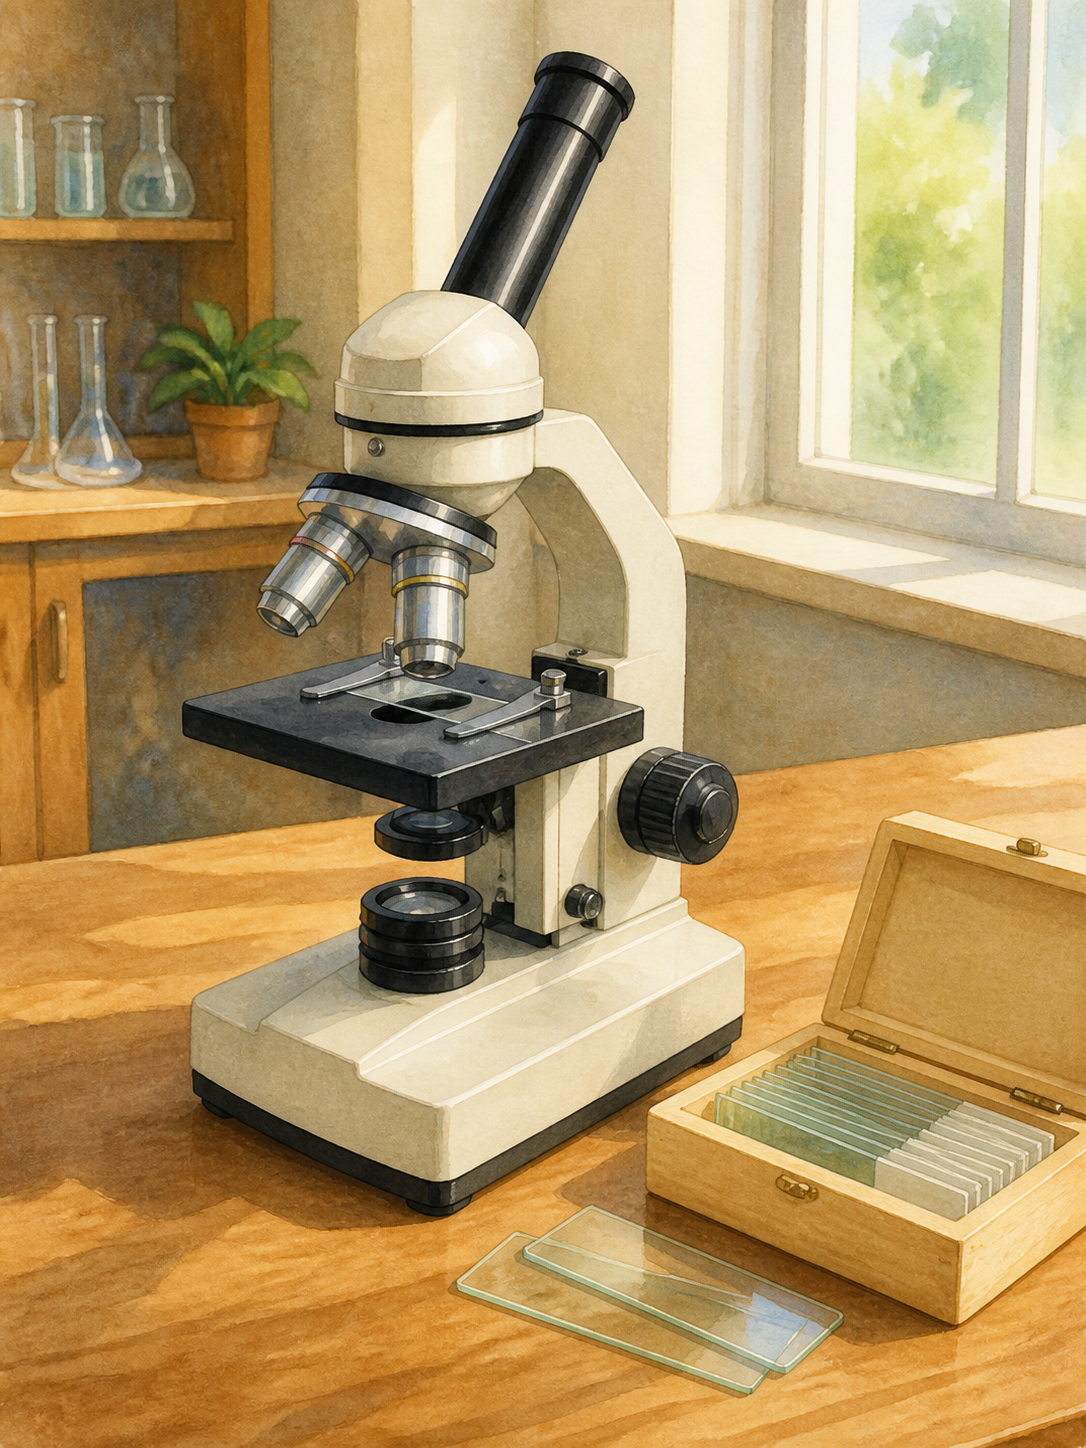
\includegraphics[width=0.44\linewidth]{images/book1/ai/g5-cells-microscope.png}

{\small الآلة التي كشفت \omterm{def:g5:first-look-at-cells:cell}{الخلايا}: عدسات، وضوء، وشريحة رقيقة على
لوح زجاجي.}
\end{omfigure}

\begin{example}[كلاسيكيتان تحت العدسة]\label{ex:g5:first-look-at-cells:classics}
رصدان يستطيع أي \omterm{def:g5:first-look-at-cells:microscope}{مجهر} مدرسي أن يعيدهما: فشظية من القشرة الرقيقة
داخل \omterm{ex:g4:plants-without-seeds:bulbtuber}{بصلة} تُظهر صفوفًا أنيقة من \omterm{def:g5:first-look-at-cells:cell}{خلايا} كالطوب، جدارًا إلى جدار؛
وكشط رفيق من باطن الخدّ يُظهر \omterm{def:g5:first-look-at-cells:cell}{خلايا} أكثر استدارة متفرقة --- وهي
خلاياك. \omterm{def:g1:plants-around-us:plant}{نبات} \omterm{def:g1:animals-around-us:animal}{وحيوان} جنبًا إلى جنب، وكلاهما خلوي.
\end{example}

\begin{omfigure}
\begin{minipage}[t]{0.48\linewidth}\centering
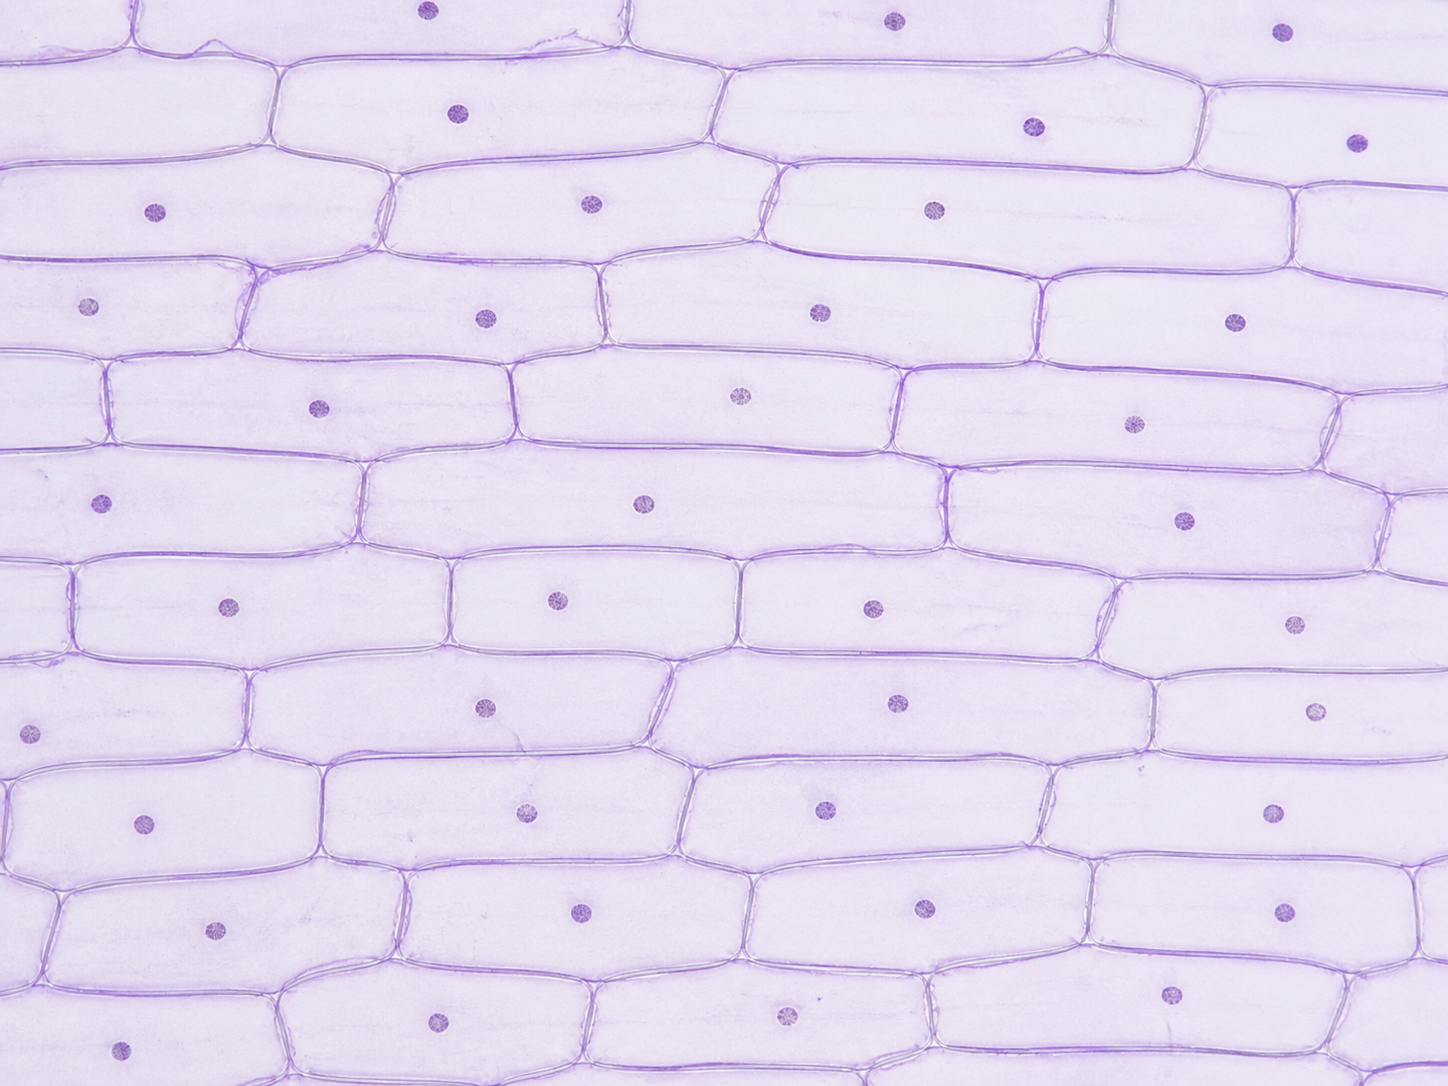
\includegraphics[width=\linewidth]{images/book1/ai/fig-onion-cells.png}

{\small قشرة \omterm{ex:g4:plants-without-seeds:bulbtuber}{البصلة}: \omterm{def:g5:first-look-at-cells:cell}{خلايا} كالطوب\\ في صفوف أنيقة}
\end{minipage}\hfill
\begin{minipage}[t]{0.48\linewidth}\centering
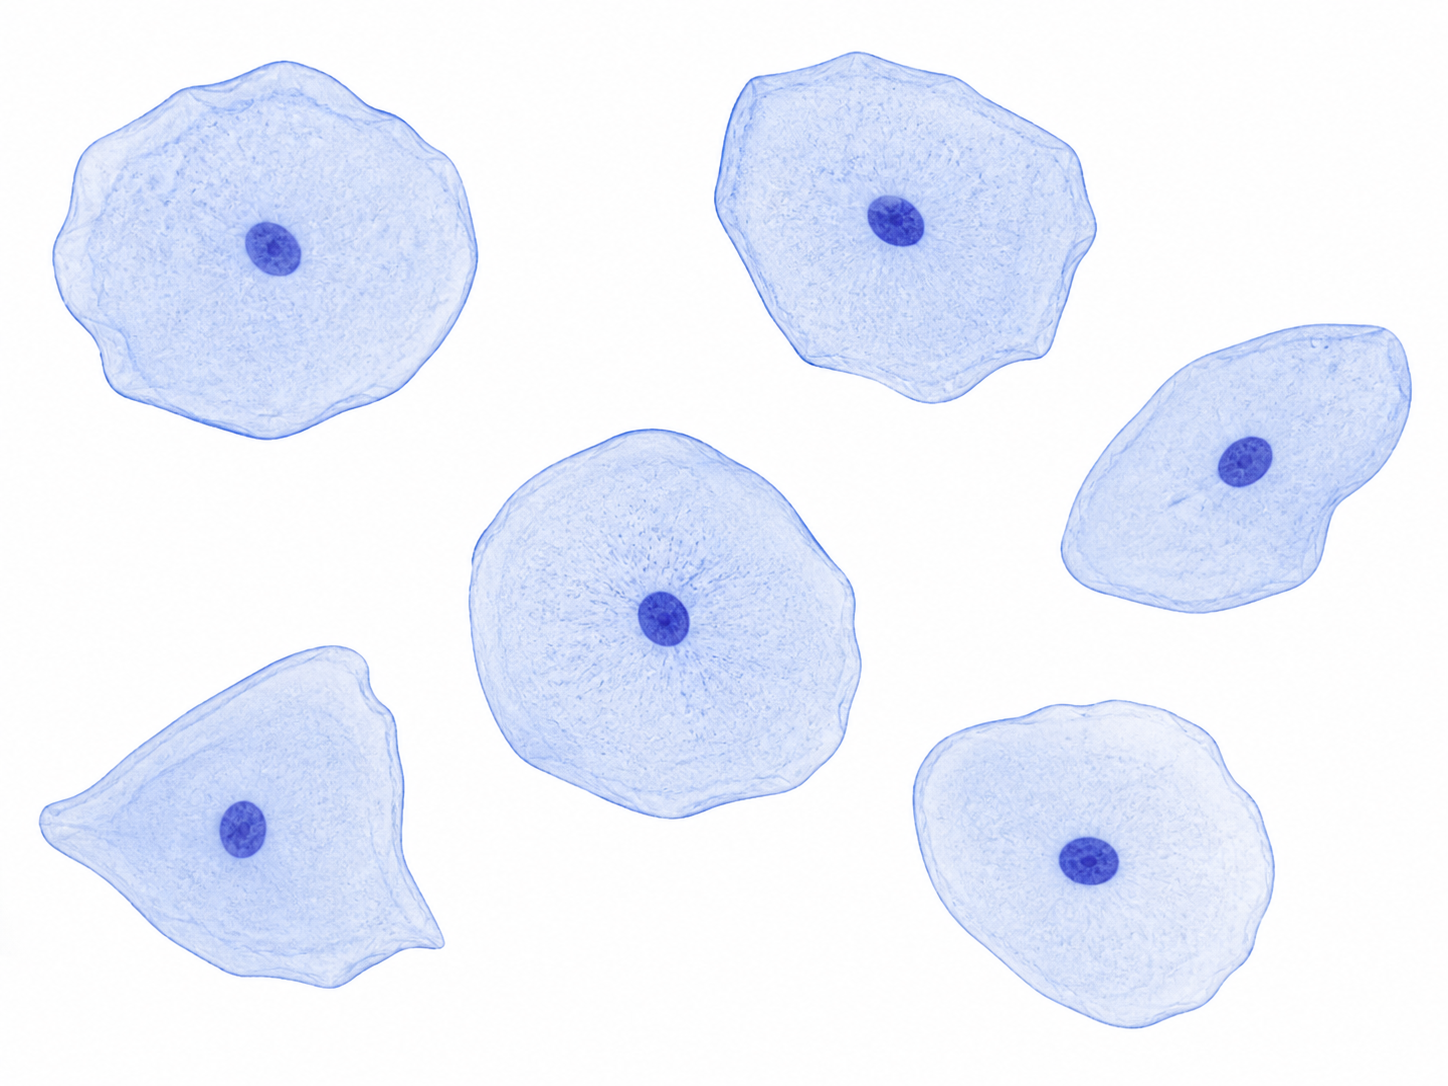
\includegraphics[width=\linewidth]{images/book1/ai/fig-cheek-cells.png}

{\small كشط الخدّ: \omterm{def:g5:first-look-at-cells:cell}{خلايا} أكثر استدارة،\\ متفرقة}
\end{minipage}

\medskip
{\small تحت \omterm{def:g5:first-look-at-cells:microscope}{المجهر}: \omterm{def:g5:first-look-at-cells:cell}{خلايا} \omterm{ex:g4:plants-without-seeds:bulbtuber}{البصلة} \omterm{def:g5:first-look-at-cells:cell}{وخلايا} الخدّ. وكل حجيرة --- ومعها
بقعتها الداكنة الصغيرة --- \omterm{def:g5:first-look-at-cells:cell}{خلية} واحدة.}
\end{omfigure}

\begin{remark}[البقعة الداكنة]\label{rem:g5:first-look-at-cells:nucleus}
في المنظرين تُظهر أكثر \omterm{def:g5:first-look-at-cells:cell}{الخلايا} بقعة أدكن صغيرة في داخلها: وهي مركز
قيادة \omterm{def:g5:first-look-at-cells:cell}{الخلية}، ويسمى \emph{النواة}\index{نواة}. أما ما تقود به
النواة --- وهو خيط التعليمات الشهير الملفوف في داخلها --- فحكاية
لسنوات هذا الكتاب اللاحقة؛ وحسبنا الآن أن نلاحظ أن الغرف الصغيرة
ليست خاوية.
\end{remark}

\section{من خلية واحدة إلى جسم}

\begin{proposition}[الأجسام تنمو بخلاياها]\label{prop:g5:first-look-at-cells:growth}
ينمو الجسم ويصلح نفسه لأن خلاياه تستطيع أن \emph{تنقسم}: فتنشطر
\omterm{def:g5:first-look-at-cells:cell}{خلية} واحدة إلى خليتين حيتين، والاثنتان إلى أربع، وهكذا. والازدياد
طولًا (\cref{prop:g3:stages-of-life:animals}) هو في أساسه تكاثر
\omterm{def:g5:first-look-at-cells:cell}{للخلايا}؛ والسحجة التي تلتئم
(\cref{rem:g3:bones-and-muscles:alive}) هي \omterm{def:g5:first-look-at-cells:cell}{خلايا} تعيد البناء. وكل
جسم، ولو كان الأكبر، بدأ \emph{\omterm{def:g5:first-look-at-cells:cell}{خلية} واحدة} --- هي \omterm{def:g4:animal-reproduction:sexual}{البويضة}
المخصَّبة في \cref{def:g4:animal-reproduction:sexual}.
\end{proposition}
\admitted

\begin{example}[من واحدة إلى تريليونات]\label{ex:g5:first-look-at-cells:one}
تنقسم \omterm{def:g4:animal-reproduction:sexual}{البويضة} المخصَّبة إلى $2$ من \omterm{def:g5:first-look-at-cells:cell}{الخلايا}، ثم إلى $4$، ثم $8$، ثم
$16$ \dots{} والانقسام المتكرر، على مدى شهور وسنوات، بنى عشرات
آلاف المليارات من \omterm{def:g5:first-look-at-cells:cell}{الخلايا} التي تقرأ هذه الجملة. وكل \omterm{def:g5:first-look-at-cells:cell}{خلية} منك تنحدر
من تلك \omterm{def:g5:first-look-at-cells:cell}{الخلية} الأولى.
\end{example}

\begin{remark}[حيوات كاملة في خلية واحدة]\label{rem:g5:first-look-at-cells:onecelled}
بعض الكائنات الحية لا يتجاوز \omterm{def:g5:first-look-at-cells:cell}{خلية} واحدة --- ولا يحتاج إلى أكثر
منها. وقطرة من ماء بركة تعجّ بها: \omterm{def:g5:first-look-at-cells:cell}{خلايا} مفردة تسبح وتتغذى وتنقسم،
حيوات كاملة على مقياس \omterm{def:g5:first-look-at-cells:microscope}{المجهر}. \omterm{def:g1:healthy-habits:germs}{وجراثيم}
\cref{def:g1:healthy-habits:germs} في أكثرها كائنات حية وحيدة
\omterm{def:g5:first-look-at-cells:cell}{الخلية} كهذه --- معارف قديمة، ولها الآن تفسير.
\end{remark}

\section{تمارين}

\begin{exercise}[$\star$]\label{exo:g5:first-look-at-cells:1}
ما \omterm{def:g5:first-look-at-cells:cell}{الخلية}؟ وكم \omterm{def:g5:first-look-at-cells:cell}{خلية} يتألف منها جسمك تقريبًا؟
\end{exercise}

\begin{exercise}[$\star$]\label{exo:g5:first-look-at-cells:2}
لماذا لم يعرف أحد شيئًا عن \omterm{def:g5:first-look-at-cells:cell}{الخلايا} في معظم التاريخ؟ وأي آلة غيّرت
ذلك؟
\end{exercise}

\begin{exercise}[$\star$]\label{exo:g5:first-look-at-cells:3}
صف ما يُظهره \omterm{def:g5:first-look-at-cells:microscope}{المجهر} في قشرة \omterm{ex:g4:plants-without-seeds:bulbtuber}{البصلة}، وفي كشط الخدّ. وبم يشترك
المنظران؟
\end{exercise}

\begin{exercise}[$\star$]\label{exo:g5:first-look-at-cells:4}
ما اسم البقعة الداكنة الصغيرة التي تُرى في أكثر \omterm{def:g5:first-look-at-cells:cell}{الخلايا}؟
\end{exercise}

\begin{exercise}[$\star$]\label{exo:g5:first-look-at-cells:5}
كم \omterm{def:g5:first-look-at-cells:cell}{خلية} من \omterm{def:g5:first-look-at-cells:cell}{خلايا} الجسم تمتد مليمترًا واحدًا إذا صُفّت --- وكم طول
\omterm{def:g5:first-look-at-cells:cell}{الخلية} الواحدة بالمليمتر؟
\end{exercise}

\begin{exercise}[$\star$]\label{exo:g5:first-look-at-cells:6}
ماذا تفعل \omterm{def:g5:first-look-at-cells:cell}{الخلايا} في الأساس حين يزداد الطفل طولًا؟ وحين تلتئم \omterm{def:g1:my-body:joint}{ركبة}
مسحوجة؟
\end{exercise}

\begin{exercise}[$\star$]\label{exo:g5:first-look-at-cells:7}
من كم \omterm{def:g5:first-look-at-cells:cell}{خلية} بدأ كل جسم بشري؟ وما تلك \omterm{def:g5:first-look-at-cells:cell}{الخلية} الأولى وفق
\cref{def:g4:animal-reproduction:sexual}؟
\end{exercise}

\begin{exercise}[$\star$]\label{exo:g5:first-look-at-cells:8}
تنقسم \omterm{def:g5:first-look-at-cells:cell}{خلية} إلى $2$؛ ثم تنقسم كل واحدة منهما من جديد، وهكذا. تابع
المضاعفة ابتداءً من $1$: كم \omterm{def:g5:first-look-at-cells:cell}{خلية} بعد $5$ انقسامات؟ وكم بعد $10$؟
\end{exercise}

\begin{exercise}[$\star\star$]\label{exo:g5:first-look-at-cells:9}
اشرح هذه الجملة: ``الأقحوانة والحوت يبينان \omterm{prop:g5:first-look-at-cells:principle}{وحدة الحياة}.'' فبم
يشتركان وفق \cref{prop:g5:first-look-at-cells:principle}؟
\end{exercise}

\begin{exercise}[$\star\star$]\label{exo:g5:first-look-at-cells:10}
قطرة من ماء بركة تحوي كائنات حية كل واحد منها \omterm{def:g5:first-look-at-cells:cell}{خلية} مفردة. راجعها
في مقابل علامات الحياة في \cref{prop:g1:living-or-not:signs}: أي
العلامات تستطيع \omterm{def:g5:first-look-at-cells:cell}{خلية} مفردة أن تُظهرها؟
\end{exercise}

\begin{exercise}[$\star\star\star$]\label{exo:g5:first-look-at-cells:11}
\omterm{def:g5:first-look-at-cells:cell}{خلايا} الفيل في حجم \omterm{def:g5:first-look-at-cells:cell}{خلايا} الفأر تقريبًا. فما الذي يجعل الفيل أكبر
إذن --- \omterm{def:g5:first-look-at-cells:cell}{خلايا} أكبر أم \omterm{def:g5:first-look-at-cells:cell}{خلايا} أكثر؟ وعلام يدل جوابك في شأن كيفية
عمل النمو، وفق \cref{prop:g5:first-look-at-cells:growth}؟
\end{exercise}
